\documentclass[a4paper,12pt]{article} % добавить leqno в [] для нумерации слева
\usepackage[a4paper,top=1.3cm,bottom=2cm,left=1.5cm,right=1.5cm,marginparwidth=0.75cm]{geometry}
%%% Работа с русским языком
\usepackage{cmap}					% поиск в PDF
\usepackage[warn]{mathtext} 		% русские буквы в фомулах
\usepackage[T2A]{fontenc}			% кодировка
\usepackage[utf8]{inputenc}			% кодировка исходного текста
\usepackage[english,russian]{babel}	% локализация и переносы
\usepackage{physics}
\usepackage{multirow}
\usepackage{bm}
\usepackage{longtable}
\usepackage{xcolor}
%%% Нормальное размещение таблиц (писать [H] в окружении таблицы)
\usepackage{float}
\restylefloat{table}


\documentclass[a4paper,12pt]{article}
\usepackage[utf8]{inputenc}
\usepackage[russian]{babel}
\usepackage{amsmath}
\usepackage{amssymb}
\usepackage{graphicx}
\usepackage{geometry}
\usepackage{booktabs}
\usepackage{caption}
\usepackage{enumitem}
\usepackage{siunitx}

\geometry{left=2cm,right=1.5cm,top=2cm,bottom=2cm}
\setlist[enumerate]{label=\arabic*., leftmargin=*}


\usepackage{graphicx}

\usepackage{wrapfig}
\usepackage{tabularx}

\usepackage{hyperref}
\usepackage[rgb]{xcolor}
\hypersetup{
	colorlinks=true,urlcolor=blue
}
\usepackage{pgfplots}
\pgfplotsset{compat=1.9}
%%% Дополнительная работа с математикой
\usepackage{amsmath,amsfonts,amssymb,amsthm,mathtools} % AMS
\usepackage{icomma} % "Умная" запятая: $0,2$ --- число, $0, 2$ --- перечисление

%% Номера формул
%\mathtoolsset{showonlyrefs=true} % Показывать номера только у тех формул, на которые есть \eqref{} в тексте,

%% Шрифты
\usepackage{euscript}	 % Шрифт Евклид
\usepackage{mathrsfs} % Красивый матшрифт

\title{Архитектура вычислительных систем. Домашнее задание №3. Вариант №1.}
\author{Комиссаров Данил Андреевич}
\date{March 2025}

\begin{document}

\section{Формальный отчет}
\begin{enumerate}
    \item Выполнил: Комиссаров Данил Андреевич.
    \item Студент группы Б01-304.
    \item Первый вариант задания.
    \item Контакты: komissarov.da@phystech.edu
    \item
\end{enumerate}
\begin{enumerate}
    \item 

\begin{figure}[H]
    \centering
    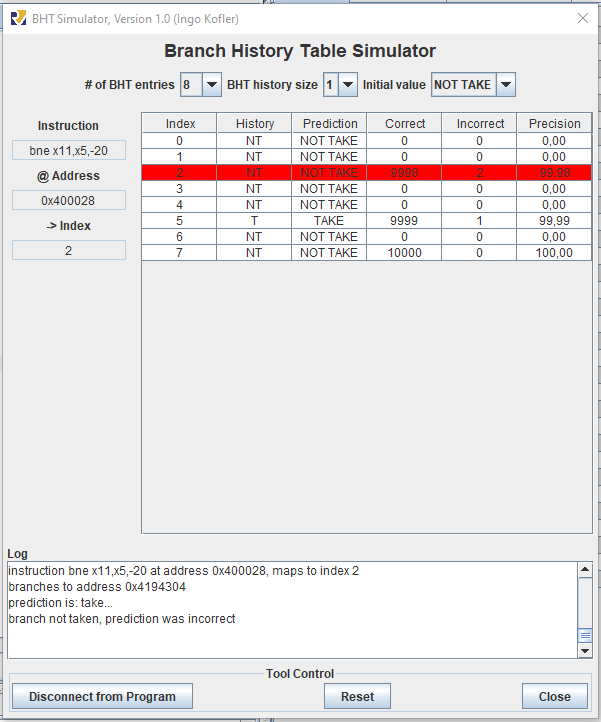
\includegraphics[width=0.75\linewidth]{Formal/BHT1.png}
\end{figure}
Точность \textbf{bagic\_br\_1} составляет 99,99\%.\\
Точность \textbf{bagic\_br\_2} составляет 100\%.
    \item 
\begin{figure}[H]
    \centering
    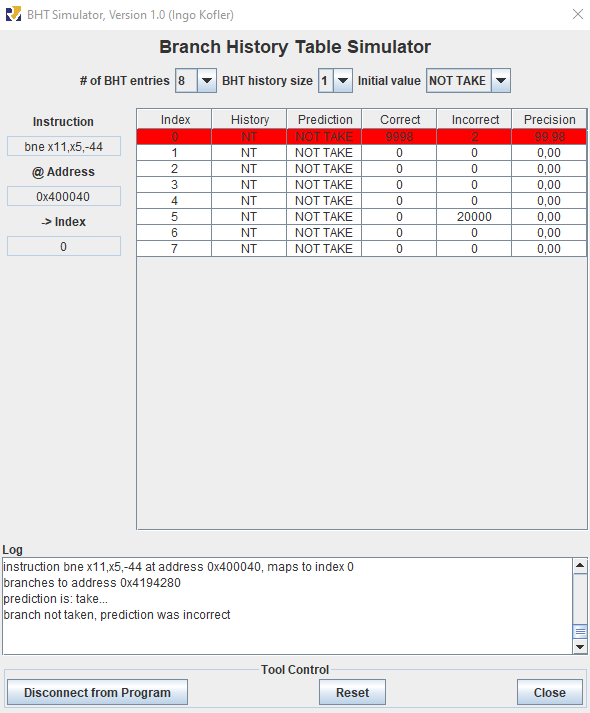
\includegraphics[width=0.75\linewidth]{Formal/BHT2.png}
\end{figure}
\begin{figure}[H]
    \centering
    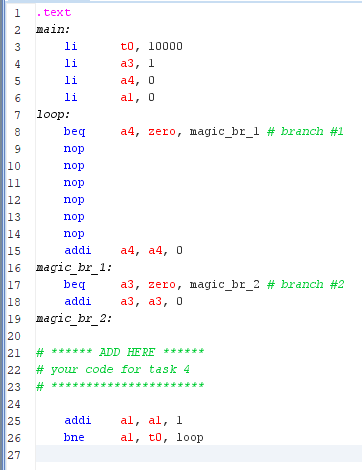
\includegraphics[width=0.5\linewidth]{Formal/task2.png}
\end{figure}
Индексы модулей предсказания для \textbf{beq} \textbf{branch1} и \textbf{branch2} совпали, а так как в настройках предиктора выставлен конечный автомат с двумя состояниями, то обманывать его можно, попеременно выдавая результаты \textit{taken} - \textit{not taken}. Так и добиваемся точности работы предиктора равной нулю.
    \item 
\begin{figure}[H]
    \centering
    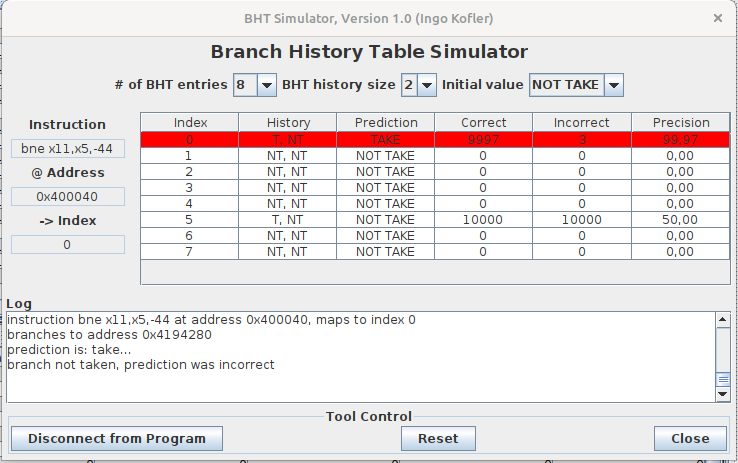
\includegraphics[width=0.75\linewidth]{Formal/BHT3.png}
\end{figure}
В отличие от предиктора из первого задания, сейчас установлен предиктор с 4 состояниями, и причем он построен так, чтобы вместо \textbf{not taken} выдавать \textbf{taken}, необходимо ошибиться 2 раза, что и происходит в цикле \textit{loop}. Так этот предиктор ошибается на 1 раз больше в цикле.
    \item 
\begin{figure}[H]
    \centering
    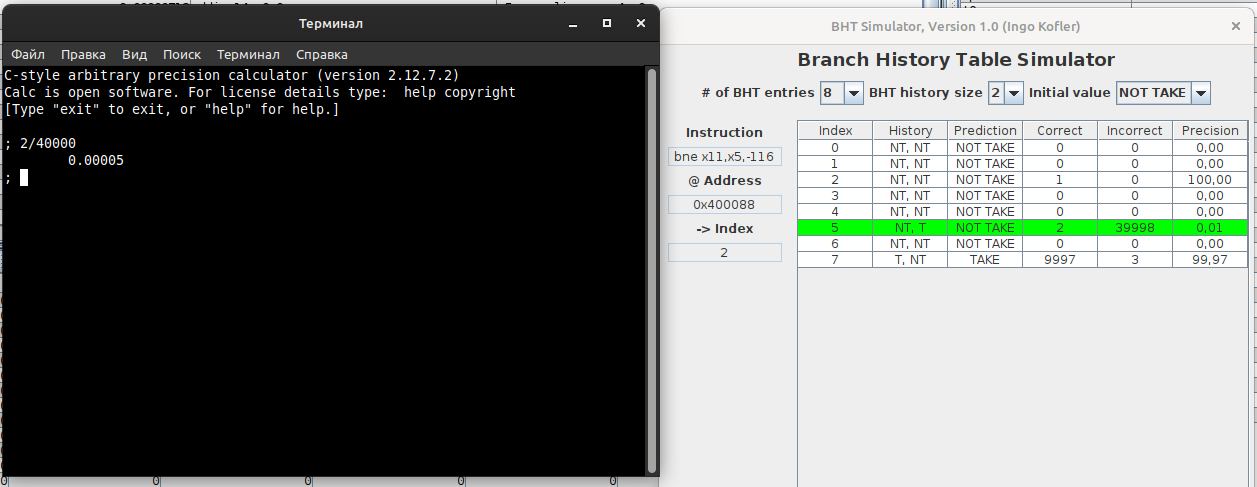
\includegraphics[width=0.75\linewidth]{Formal/BHT4.png}
\end{figure}
\begin{figure}[H]
    \centering
    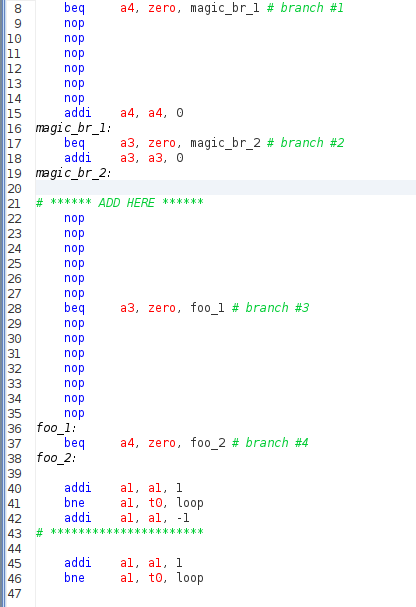
\includegraphics[width=0.75\linewidth]{Formal/task4.png}
\end{figure}
Действительно, так и сделаем: цикл \textbf{taken} - \textbf{taken} - \textbf{not taken} - \textbf{not taken}.
В конце концов на ассемблере пишем, даже внутри ограниченного пространства можем перелопатить программу до неузнаваемости. Корректно процент предсказания уже не прописывается в программе, считаем отдельно в калькуляторе. Увеличивая начальное значение \textbf{t0}, уменьшается процент предсказания, но я не стал увеличивать, так как комп не тянет. 
\end{enumerate}
\end{document}